\documentclass{article}
\usepackage[utf8]{inputenc}
\usepackage[T1]{fontenc}
\usepackage{booktabs}
\usepackage{geometry}
\usepackage{amsmath}
\usepackage{graphicx}
% Use xurl to ensure links break properly across lines in footnotes
\usepackage{tablefootnote}
\usepackage{xurl} 
\usepackage[colorlinks=true, allcolors=blue, breaklinks=true]{hyperref}

\geometry{margin=1in}

\title{Architecture and Cost-Benefit Analysis of a High-Precision Synchronized SDR System}
\author{RF Research Department}
\date{\today}

\begin{document}

\maketitle

\begin{abstract}
This document outlines the technical specifications, Bill of Materials (BOM), and design trade-offs for a software-defined radio (SDR) system optimized for phase-coherent applications, such as direction finding and precision signal acquisition. The architecture integrates an Analog Devices AD936x-based transceiver with a Jetson Nano for edge processing, utilizing a GPS-Disciplined Oscillator (GPSDO) to ensure frequency stability and temporal alignment via 1 PPS and 10 MHz reference signals.
\end{abstract}

\section{System Architecture}
\begin{figure}[h]
    \centering
    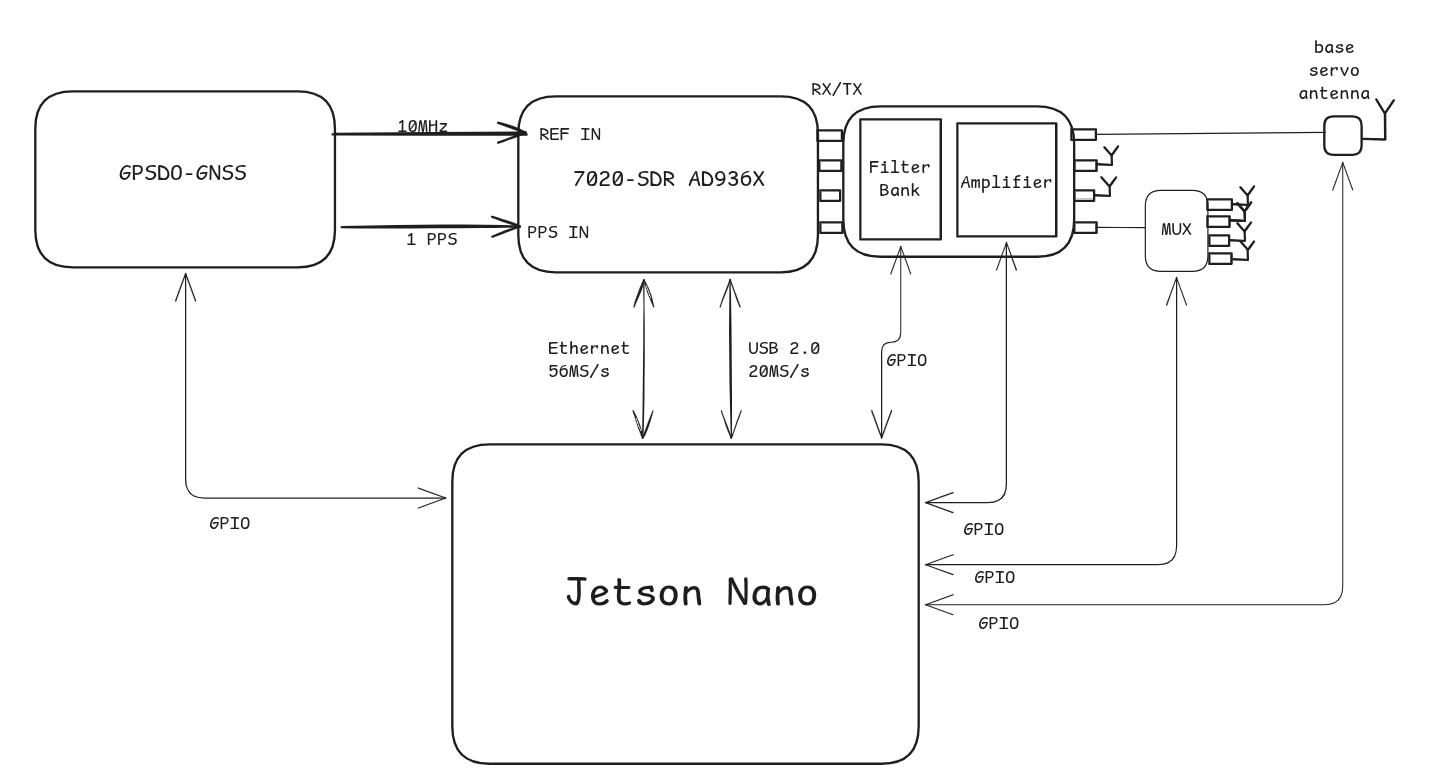
\includegraphics[width=0.8\textwidth]{images/Diagram.png}
    \caption{Functional Block Diagram: Synchronized SDR with RF Front-End and Edge Compute.}
\end{figure}

\section{Bill of Materials (BOM)}
The following table provides the components required for two distinct configurations. All prices are in USD and were verified on February 3, 2026.

\begin{table}[h]
\centering
\small
\begin{tabular}{@{}p{3.5cm}p{6cm}rr@{}}
\toprule
\textbf{Component} & \textbf{Technical Justification} & \textbf{Price (USD)} & \textbf{Ref.} \\ \midrule

\textbf{SDR (Entry-Level)} &
Nooelec NESDR Smart v5: Reliable wideband receiver (100kHz–1.75GHz). &
\$42.95 &
\tablefootnote{Amazon, Feb 3, 2026.
\url{https://www.amazon.com/Nooelec-RTL-SDR-SDR-100kHz-1-75GHz-Enclosure/dp/B01HA642SW}}
\\

\textbf{SDR (Research-Grade)} &
OpenSourceSDRLab 7020-SDR AD9361: Zynq 7020 based platform with MIMO. &
\$498.00 &
\tablefootnote{OpenSourceSDRLab, Feb 3, 2026.
\url{https://opensourcesdrlab.com/products/opensourcesdrlab-new-7020-sdr-ad9361-development-board-with-pa-for-pluto-sdr-matlab-software-defined-radio?VariantsId=10346}}
\\

\textbf{LNA (Front-end)} &
Nooelec LaNA: Wideband Low-Noise Amplifier (20MHz–4GHz). &
\$29.95 &
\tablefootnote{Nooelec, Feb 3, 2026.
\url{https://www.nooelec.com/store/lana.html}}
\\

\textbf{GPSDO Reference} &
Leo Bodnar Mini GPSDO: Ultra-stable 10 MHz reference. &
\$125.00 &
\tablefootnote{Leo Bodnar, Feb 3, 2026.
\url{https://www.leobodnar.com/shop/index.php?main_page=product_info&cPath=107&products_id=393}}
\\

\textbf{Antenna (General)} &
Wideband Log-Periodic (600 MHz–6 GHz) for survey work. &
\$45.00 &
\tablefootnote{Generic RF supplier average price, Feb 2026.}
\\

\textbf{Servo Antenna Base} &
Pan-Tilt Servo mechanism for directional tracking. &
\$150.00 &
\tablefootnote{Estimated price for precision metal-gear kit, Feb 2026.}
\\

\textbf{Support Hardware} &
SMA Cables, 5V/4A Power Supply, and GPIO Breakouts. &
\$80.00 &
\tablefootnote{Estimated based on current hardware listings.}
\\

\bottomrule
\end{tabular}
\end{table}

\subsection{Cost Summation}
\begin{itemize}
    \item \textbf{Entry-Level Configuration Total:} \$472.90
    \item \textbf{Research-Grade Configuration Total:} \$927.95
\end{itemize}

\section{Design Purpose}
This system is designed for **Radio Frequency Interference (RFI) Localization** and **Time Difference of Arrival (TDOA)** research. By utilizing the 1 PPS signal from the GPSDO, the system can timestamp IQ samples with nanosecond precision.

\section{Weaknesses and Limitations}
\begin{enumerate}
    \item \textbf{Dynamic Range:} The AD9361 uses a 12-bit ADC.
    \item \textbf{Host Compute Dependency:} Jetson Nano throughput limitations over USB 2.0.
    \item \textbf{Calibration:} Phase coherence requires periodic thermal calibration.
    \item \textbf{Susceptibility:} Servo motor EMI requires shielding.
\end{enumerate}

\section{Assumptions and Verifications}
\begin{itemize}
    \item \textbf{Prices:} Market listings as of February 2026.
    \item \textbf{Specifications:} Bandwidth limits are based on hardware bus capabilities.
\end{itemize}

\end{document}